\documentclass{standalone}
\usepackage{tikz}
\usetikzlibrary{patterns, positioning}

\begin{document}
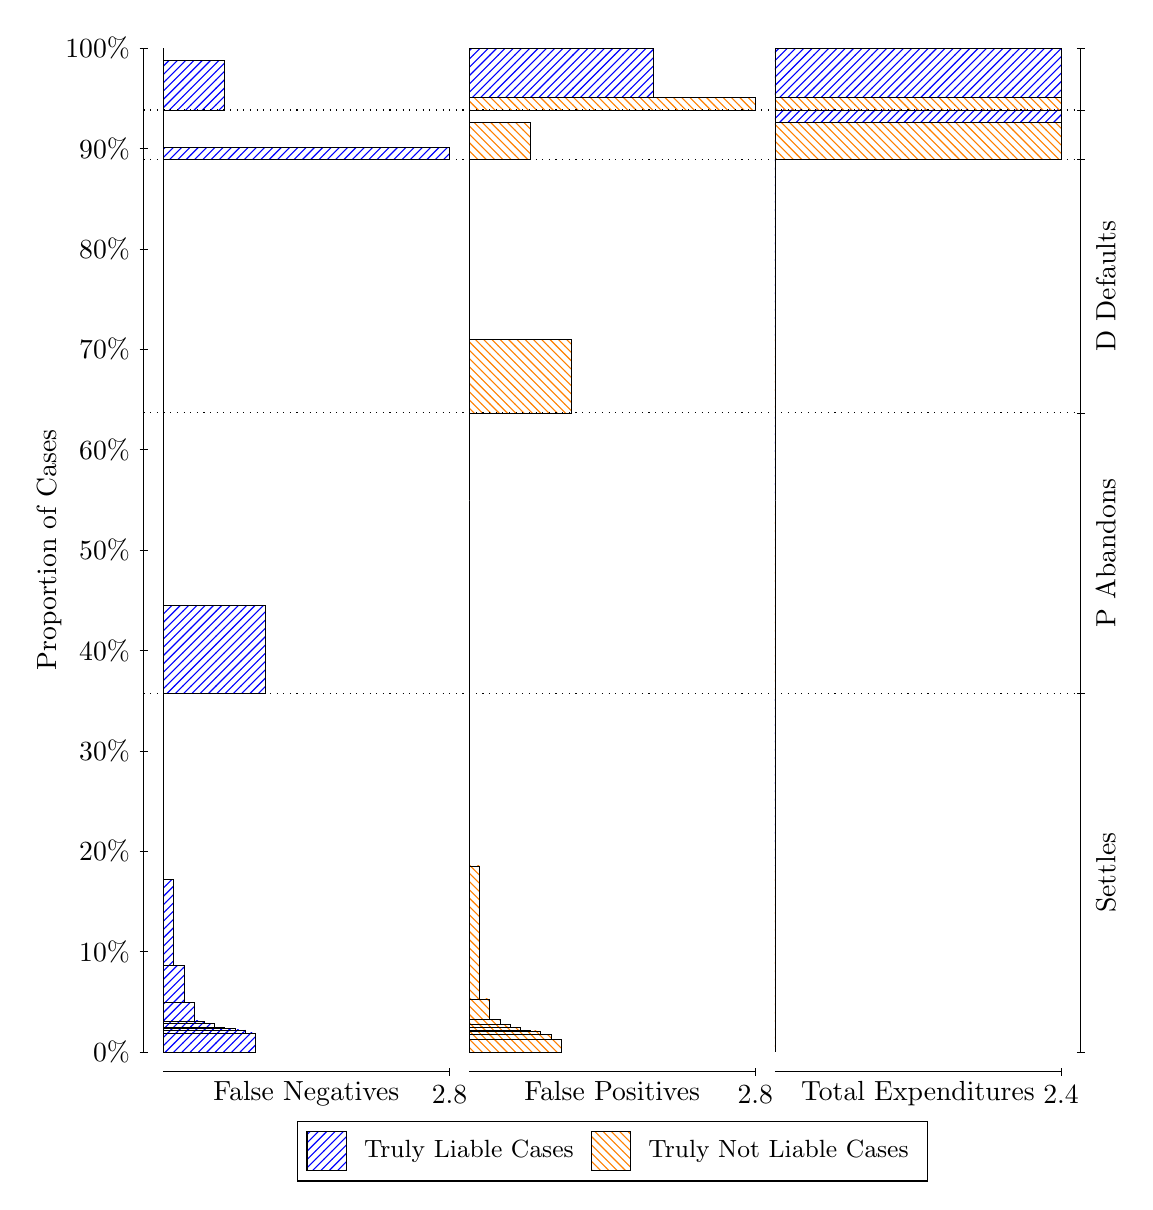
\begin{tikzpicture}
\draw[black, very thin] (1.5,1.75) -- (1.5,14.5);
\node[rotate=90, anchor=center] at (0.3, 8.125) {Proportion of Cases};
\draw[black, very thin] (1.45,1.75) -- (1.55,1.75);
\node[anchor=east] at (1.45, 1.75) {0\%};
\draw[black, very thin] (1.45,3.025) -- (1.55,3.025);
\node[anchor=east] at (1.45, 3.025) {10\%};
\draw[black, very thin] (1.45,4.3) -- (1.55,4.3);
\node[anchor=east] at (1.45, 4.3) {20\%};
\draw[black, very thin] (1.45,5.575) -- (1.55,5.575);
\node[anchor=east] at (1.45, 5.575) {30\%};
\draw[black, very thin] (1.45,6.85) -- (1.55,6.85);
\node[anchor=east] at (1.45, 6.85) {40\%};
\draw[black, very thin] (1.45,8.125) -- (1.55,8.125);
\node[anchor=east] at (1.45, 8.125) {50\%};
\draw[black, very thin] (1.45,9.4) -- (1.55,9.4);
\node[anchor=east] at (1.45, 9.4) {60\%};
\draw[black, very thin] (1.45,10.675) -- (1.55,10.675);
\node[anchor=east] at (1.45, 10.675) {70\%};
\draw[black, very thin] (1.45,11.95) -- (1.55,11.95);
\node[anchor=east] at (1.45, 11.95) {80\%};
\draw[black, very thin] (1.45,13.225) -- (1.55,13.225);
\node[anchor=east] at (1.45, 13.225) {90\%};
\draw[black, very thin] (1.45,14.5) -- (1.55,14.5);
\node[anchor=east] at (1.45, 14.5) {100\%};

\draw[black, very thin] (13.4,1.75) -- (13.4,14.5);
\draw[black, very thin] (13.35,1.75) -- (13.45,1.75);
\node[anchor=west] at (13.35, 1.75) {};
\draw[black, very thin] (13.35,6.3055) -- (13.45,6.3055);
\node[anchor=west] at (13.35, 6.3055) {};
\draw[black, very thin] (13.35,9.8666) -- (13.45,9.8666);
\node[anchor=west] at (13.35, 9.8666) {};
\draw[black, very thin] (13.35,13.086) -- (13.45,13.086);
\node[anchor=west] at (13.35, 13.086) {};
\draw[black, very thin] (13.35,13.713) -- (13.45,13.713);
\node[anchor=west] at (13.35, 13.713) {};
\draw[black, very thin] (13.35,14.5) -- (13.45,14.5);
\node[anchor=west] at (13.35, 14.5) {};

\draw[black, very thin, pattern color=blue, pattern=north east lines] (1.75,1.75) rectangle (2.9179,1.9915);
\draw[black, very thin, pattern color=blue, pattern=north east lines] (1.75,1.9915) rectangle (2.7881,2.0297);
\draw[black, very thin, pattern color=blue, pattern=north east lines] (1.75,2.0297) rectangle (2.6583,2.0472);
\draw[black, very thin, pattern color=blue, pattern=north east lines] (1.75,2.0472) rectangle (2.5286,2.0643);
\draw[black, very thin, pattern color=blue, pattern=north east lines] (1.75,2.0643) rectangle (2.5286,2.066);
\draw[black, very thin, pattern color=blue, pattern=north east lines] (1.75,2.066) rectangle (2.3988,2.1105);
\draw[black, very thin, pattern color=blue, pattern=north east lines] (1.75,2.1105) rectangle (2.269,2.1442);
\draw[black, very thin, pattern color=blue, pattern=north east lines] (1.75,2.1442) rectangle (2.1393,2.3822);
\draw[black, very thin, pattern color=blue, pattern=north east lines] (1.75,2.3822) rectangle (2.0095,2.8518);
\draw[black, very thin, pattern color=blue, pattern=north east lines] (1.75,2.8518) rectangle (1.8798,3.9411);
\draw[black, very thin, pattern color=orange, pattern=north west lines] (1.75,3.9411) rectangle (1.75,6.3055);
\draw[black, very thin, pattern color=blue, pattern=north east lines] (1.75,6.3055) rectangle (3.0476,7.4189);
\draw[black, very thin, pattern color=orange, pattern=north west lines] (1.75,7.4189) rectangle (1.75,9.8666);
\draw[black, very thin, pattern color=orange, pattern=north west lines] (1.75,9.8666) rectangle (1.75,10.802);
\draw[black, very thin, pattern color=blue, pattern=north east lines] (1.75,10.802) rectangle (1.75,13.086);
\draw[black, very thin, pattern color=blue, pattern=north east lines] (1.75,13.086) rectangle (5.3833,13.241);
\draw[black, very thin, pattern color=orange, pattern=north west lines] (1.75,13.241) rectangle (1.75,13.713);
\draw[black, very thin, pattern color=blue, pattern=north east lines] (1.75,13.713) rectangle (2.5286,14.344);
\draw[black, very thin, pattern color=orange, pattern=north west lines] (1.75,14.344) rectangle (1.75,14.5);
\draw[black, very thin, pattern color=orange, pattern=north west lines] (5.6333,1.75) rectangle (6.8012,1.9065);
\draw[black, very thin, pattern color=orange, pattern=north west lines] (5.6333,1.9065) rectangle (6.6714,1.9736);
\draw[black, very thin, pattern color=orange, pattern=north west lines] (5.6333,1.9736) rectangle (6.5417,2.0179);
\draw[black, very thin, pattern color=orange, pattern=north west lines] (5.6333,2.0179) rectangle (6.4119,2.0285);
\draw[black, very thin, pattern color=orange, pattern=north west lines] (5.6333,2.0285) rectangle (6.2821,2.0662);
\draw[black, very thin, pattern color=orange, pattern=north west lines] (5.6333,2.0662) rectangle (6.1524,2.07);
\draw[black, very thin, pattern color=orange, pattern=north west lines] (5.6333,2.07) rectangle (6.1524,2.0962);
\draw[black, very thin, pattern color=orange, pattern=north west lines] (5.6333,2.0962) rectangle (6.0226,2.1636);
\draw[black, very thin, pattern color=orange, pattern=north west lines] (5.6333,2.1636) rectangle (5.8929,2.4249);
\draw[black, very thin, pattern color=orange, pattern=north west lines] (5.6333,2.4249) rectangle (5.7631,4.1143);
\draw[black, very thin, pattern color=blue, pattern=north east lines] (5.6333,4.1143) rectangle (5.6333,6.3055);
\draw[black, very thin, pattern color=orange, pattern=north west lines] (5.6333,6.3055) rectangle (5.6333,8.7532);
\draw[black, very thin, pattern color=blue, pattern=north east lines] (5.6333,8.7532) rectangle (5.6333,9.8666);
\draw[black, very thin, pattern color=orange, pattern=north west lines] (5.6333,9.8666) rectangle (6.931,10.802);
\draw[black, very thin, pattern color=blue, pattern=north east lines] (5.6333,10.802) rectangle (5.6333,13.086);
\draw[black, very thin, pattern color=orange, pattern=north west lines] (5.6333,13.086) rectangle (6.4119,13.558);
\draw[black, very thin, pattern color=blue, pattern=north east lines] (5.6333,13.558) rectangle (5.6333,13.713);
\draw[black, very thin, pattern color=orange, pattern=north west lines] (5.6333,13.713) rectangle (9.2667,13.869);
\draw[black, very thin, pattern color=blue, pattern=north east lines] (5.6333,13.869) rectangle (7.969,14.5);
\draw[black, very thin, pattern color=orange, pattern=north west lines] (9.5167,1.75) rectangle (9.5167,4.1143);
\draw[black, very thin, pattern color=blue, pattern=north east lines] (9.5167,4.1143) rectangle (9.5167,6.3055);
\draw[black, very thin, pattern color=orange, pattern=north west lines] (9.5167,6.3055) rectangle (9.5167,8.7532);
\draw[black, very thin, pattern color=blue, pattern=north east lines] (9.5167,8.7532) rectangle (9.5167,9.8666);
\draw[black, very thin, pattern color=orange, pattern=north west lines] (9.5167,9.8666) rectangle (9.5167,10.802);
\draw[black, very thin, pattern color=blue, pattern=north east lines] (9.5167,10.802) rectangle (9.5167,13.086);
\draw[black, very thin, pattern color=orange, pattern=north west lines] (9.5167,13.086) rectangle (13.15,13.558);
\draw[black, very thin, pattern color=blue, pattern=north east lines] (9.5167,13.558) rectangle (13.15,13.713);
\draw[black, very thin, pattern color=orange, pattern=north west lines] (9.5167,13.713) rectangle (13.15,13.869);
\draw[black, very thin, pattern color=blue, pattern=north east lines] (9.5167,13.869) rectangle (13.15,14.5);
\draw[black, dotted] (1.5,6.3055) -- (13.4,6.3055);
\draw[black, dotted] (1.5,9.8666) -- (13.4,9.8666);
\draw[black, dotted] (1.5,13.086) -- (13.4,13.086);
\draw[black, dotted] (1.5,13.713) -- (13.4,13.713);
\draw[black, very thin] (1.75,1.5) -- (5.3833,1.5);
\node[anchor=north] at (3.5667, 1.5) {False Negatives};
\draw[black, very thin] (5.3833,1.45) -- (5.3833,1.55);
\node[anchor=north] at (5.3833, 1.45) {2.8};

\draw[black, very thin] (5.6333,1.5) -- (9.2667,1.5);
\node[anchor=north] at (7.45, 1.5) {False Positives};
\draw[black, very thin] (9.2667,1.45) -- (9.2667,1.55);
\node[anchor=north] at (9.2667, 1.45) {2.8};

\draw[black, very thin] (9.5167,1.5) -- (13.15,1.5);
\node[anchor=north] at (11.333, 1.5) {Total Expenditures};
\draw[black, very thin] (13.15,1.45) -- (13.15,1.55);
\node[anchor=north] at (13.15, 1.45) {2.4};

\node[black, centered, rotate=90] at (13.72, 4.0277) {Settles};
\node[black, centered, rotate=90] at (13.72, 8.086) {P Abandons};
\node[black, centered, rotate=90] at (13.72, 11.476) {D Defaults};



\draw (7.449999999999999,1.5) node[draw=none] (baseCoordinate) {};
\begin{scope}[align=center]
        \matrix[scale=0.5, draw=black, below=0.5cm of baseCoordinate, nodes={draw}, column sep=0.1cm]{
            \node[rectangle, draw, minimum width=0.5cm, minimum height=0.5cm, pattern=north east lines, pattern color=blue] {}; &
            \node[draw=none, font=\small] (B) {Truly Liable Cases}; &
            \node[rectangle, draw, minimum width=0.5cm, minimum height=0.5cm, pattern=north west lines, pattern color=orange] {}; &
            \node[draw=none, font=\small] (B) {Truly Not Liable Cases}; \\
            };
\end{scope}

\end{tikzpicture}
\end{document}